\documentclass[a4paper,12pt]{article}

\usepackage[utf8]{inputenc}
\usepackage[english]{babel}
\usepackage[T1]{fontenc} % for correct << and >>
\usepackage{amssymb, amsmath, multicol, amsthm, mathtools}
\usepackage{csquotes}
\usepackage{mathrsfs}
\usepackage{graphicx}
\usepackage{multirow}
\usepackage{caption}
\usepackage{subcaption}
\usepackage{indentfirst}
\usepackage{esvect}
\usepackage{float} 
\usepackage[version=4]{mhchem}
\mathtoolsset{showonlyrefs=true}
\usepackage{hyperref}
\usepackage[rgb,table,xcdraw]{xcolor}
\hypersetup{				
	unicode=true,        
	colorlinks=true,       	
	linkcolor=black,        
	citecolor=black,        
	filecolor=magenta,      
	urlcolor=black         
}
\usepackage{pythonhighlight}

\usepackage[left=2cm,right=2cm,
    top=2cm,bottom=2cm]{geometry}
\usepackage{fancyhdr}


\graphicspath{{images}}

\newcommand{\angstrom}{\text{\normalfont\AA}}
\newcommand{\iu}{\mathrm{i}\mkern1mu}
\newcommand*{\hatH}{\hat{\mathcal{H}}}





\begin{document}

    \begin{center}
    \centering \LARGE SpinW factor 2 problem

    \vspace{1cm}
    \small Andrey Rybakov and Marko Marino
    \end{center}

    \section{The problem}

        SpinW \cite{SpinW} results does not reproduce the test case of 1D ferromagnetic chain, neither 3D ferromagnetic cubic crystal. 
        The magnon dispersion for such systems plotted with SpinW is twice as small as the result from textbooks 
        \cite{rezende2020fundamentals, blundell2003magnetism, gurevich1996magnetization, simon2013oxford, coey2010magnetism, jensen1991rare} (conversion from textbook's notations are discussed in Appendix~I). 

        Since there are various notations for the Spin Hamiltonian, which is the starting point for the magnon dispersion calculation, 
        in this paper all results are presents with respect to the notation of SpinW paper \cite{toth2015linear}:

        \begin{equation}
            H = \sum_{mi,nj}\boldsymbol{S}^T_{mi}\boldsymbol{J}_{mi, nj}\boldsymbol{S}_{nj} + 
            \sum_{mi}\boldsymbol{S}^T_{mi}\boldsymbol{A}_{mi}\boldsymbol{S}_{mi} + 
            \mu_B\boldsymbol{H}^T\sum_{mi}g_i\boldsymbol{S}_{mi},
        \end{equation}
        where double counting is present in the sum and negative $J$ means ferromagnetic alignment. 
        First term descries exchange interaction, second -- single ion anisotropy, third -- external magnetic field.
        The indices $m$, $n$ are indexing the crystallographic unit cell (running from $1$ to $L$), while $i$ and $j$ label the magnetic atoms inside unit cell (running from $1$ to $N$).
        $\boldsymbol{S}_i$ is a $3 \times 1$ column vector of spin operators $\{S_{mi}^x, S_{mi}^y, S_{mi}^z\}$, 
        $\boldsymbol{J}_{mi, nj}$ is a matrix of exchange parameters, $\boldsymbol{A}_{mi}$ - matrix of single ion anisotropy,  
        $\boldsymbol{H}$ - column vector of external magnetic field. 

        For the ferromagnetic 3D crystal with one magnetic center in unit cell the solution of SpinW gives:

        \begin{equation}
            E(\boldsymbol{k}) = \hbar\omega(\boldsymbol{k}) = SJn\left(\dfrac{1}{3}\left(\cos(k_xl) + \cos(k_yl) + \cos(k_zl)\right) - 1\right),
        \end{equation}
        where $l$ is the length of lattice parameters. While the textbook's results gives for the same system:
        \begin{equation}
            E(\boldsymbol{k}) = \hbar\omega(\boldsymbol{k}) = 2SJn\left(\dfrac{1}{3}\left(\cos(k_xl) + \cos(k_yl) + \cos(k_zl)\right) - 1\right). \label{eq:textbook}
        \end{equation}

        In the Fig.~\ref{fig:dispersion-comparasion} The magnon dispersion is plotted for both solutions along the k-path specified in \cite{setyawan2010high}, $J = 1$, $S = 1$, $n = 6$.

        \begin{figure}[H]
            \centering
            \begin{subfigure}[b]{0.8\textwidth}
                \centering
                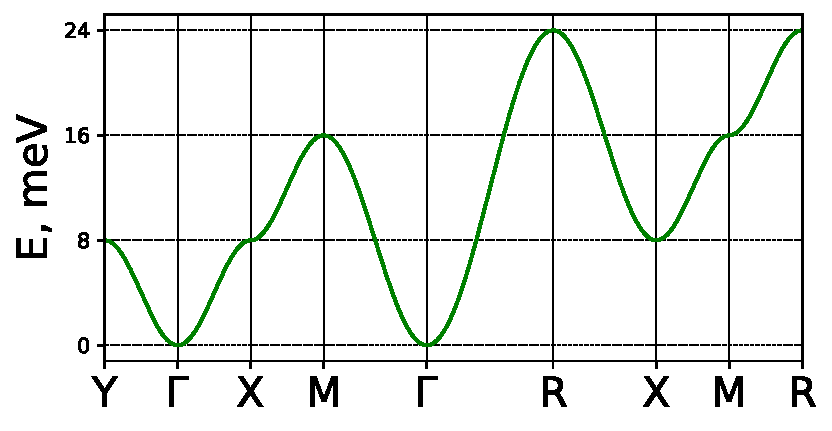
\includegraphics[height=6cm]{main_dispersion.pdf}
            \end{subfigure}
            \hfill
            \caption{Magnon dispersion comparison between SpinW and textbooks ($J = 1$, $S = 1$).}
            \label{fig:dispersion-comparasion}
        \end{figure}

        In the SpinW paper \cite{toth2015linear} the solution starts by the two consecutive rotations, 
        which results in the rotation of the exchange matrix $\boldsymbol{J}^{\prime}_{mi, nj} = \boldsymbol{J}_{mi, nj}\boldsymbol{R}_{n-m}$ 
        the definition of the vectors $\boldsymbol{u}$ and $\boldsymbol{v}$.
        This rotation does not affect the following discussion, therefore we drop the $^{\prime}$ sign in the $\boldsymbol{J}_{mi, nj}$ 
        and use the complex valued vectors $\boldsymbol{u}$ and $\boldsymbol{v}$, without recalling their definition here. 
        The unique comment that is important here is that for ferromagnetic case (oriented along $z$ axis) the values of the vectors are:
        \begin{equation}
            \boldsymbol{u} = (1, i, 0)^T
        \end{equation}
        \begin{equation}
            \boldsymbol{v} = (0, 0, 1)^T
        \end{equation}

        The single-ion anisotropy term and magnetic field term can be merged into the exchange term as explained in the SpinW paper \cite{toth2015linear}.

    \section{The solution}

    Starting point for the following discussion is equation (20) from the SpinW paper \cite{toth2015linear} 
    (adjusted with respect to the comment at the end of the previous section):

    \begin{multline}
        H = \sum_{mi, nj}\left\{\sqrt{\dfrac{S_{i}}{2}}\left(\overline{\boldsymbol{u}}^T_i b_{mi} + \boldsymbol{u}^T_i b^{\dag}_{mi} \right) + 
        \boldsymbol{v}^T_i(S_i - b^{\dag}_{mi}b_{mi})\right\}  \cdot
        \boldsymbol{J}_{mi, nj}\\
        \cdot\left\{\sqrt{\dfrac{S_{j}}{2}}\left(\overline{\boldsymbol{u}}_j b_{nj} + \boldsymbol{u}_j b^{\dag}_{nj} \right) + 
        \boldsymbol{v}_j(S_j - b^{\dag}_{nj}b_{nj})\right\},
    \end{multline}
    where $b^{\dag}_{mi}$ and $b_{mi}$ are the creation and annihilation operators of the local quantum spin deviations. Overline denotes complex conjugate.

    After the expansion the Hamiltonian Has the zero energy term $E_0$, the term with one-operator terms, expectation value of which vanishes. 
    And the two-operator term $H^{(2)}$, which is the center of attention in linearised spin-wave theory. 
    We focus on this term, taking into account the property of the exchange matrix $\boldsymbol{J}_{mi, nj} = \boldsymbol{J}_{i,j}(d)$, $\boldsymbol{d} = \boldsymbol{r}_n - \boldsymbol{r}_m$:
    \begin{multline}
        H^{(2)} = \dfrac{\sqrt{S_i S_j}}{2}\left(\overline{\boldsymbol{u}}^T_i\boldsymbol{J}_{i,j}(\boldsymbol{d})\overline{\boldsymbol{u}}_jb_{mi}b_{nj} +
        \overline{\boldsymbol{u}}^T_i\boldsymbol{J}_{i,j}(\boldsymbol{d})\boldsymbol{u}_j b_{mi}b^{\dag}_{nj}\right. \\+ 
        \left.\boldsymbol{u}^T_i\boldsymbol{J}_{i,j}(\boldsymbol{d})\overline{\boldsymbol{u}}_jb^{\dag}_{mi}b_{nj} +
        \boldsymbol{u}^T_i\boldsymbol{J}_{i,j}(\boldsymbol{d})\boldsymbol{u}_jb^{\dag}_{mi}b^{\dag}_{nj}\right) \\-
        \boldsymbol{v}^T_i\boldsymbol{J}_{i,j}(\boldsymbol{d})\boldsymbol{v}_j\left(S_ib^{\dag}_{nj}b_{nj} + S_jb^{\dag}_{mi}b_{mi}\right)
    \end{multline}

    The next step of the solution is to apply Fourier transformation in order to move from the creation and annihilation operators 
    of the local quantum spin deviations ($b^{\dag}_{mi}$ and $b_{mi}$) 
    to the creation and annihilation operators of collective quantum excitations ($b^{\dag}(k)$ and $b(k)$).
    \begin{equation}
        b_{mi} = \dfrac{1}{\sqrt{L}}\sum_{\boldsymbol{k} \in \text{B.Z.}} b_i(\boldsymbol{k})e^{i\boldsymbol{k}\boldsymbol{r}_m},
    \end{equation}
    \begin{equation}
        b^{\dag}_{mi} = \dfrac{1}{\sqrt{L}}\sum_{\boldsymbol{k} \in \text{B.Z.}} b^{\dag}_i(\boldsymbol{k})e^{-i\boldsymbol{k}\boldsymbol{r}_m},
    \end{equation}

    After the Fourier transformation the Hamiltonian has the form:
    \begin{multline}
        H^{(2)} = \sum_{ij}\sum_{\boldsymbol{k}}\left[\dfrac{\sqrt{S_i S_j}}{2}\overline{\boldsymbol{u}}^T_i\boldsymbol{J}_{i,j}(\boldsymbol{k})\overline{\boldsymbol{u}}_jb_{i}(\boldsymbol{k})b_{j}(-\boldsymbol{k}) +
        \dfrac{\sqrt{S_i S_j}}{2} \overline{\boldsymbol{u}}^T_i\boldsymbol{J}_{i,j}(\boldsymbol{k})\boldsymbol{u}_j b_{i}(\boldsymbol{k})b^{\dag}_{j}(\boldsymbol{k})\right. \\+ 
        \dfrac{\sqrt{S_i S_j}}{2}\boldsymbol{u}^T_i\boldsymbol{J}_{i,j}(-\boldsymbol{k})\overline{\boldsymbol{u}}_jb^{\dag}_{i}(\boldsymbol{k})b_{j}(\boldsymbol{k}) +
        \dfrac{\sqrt{S_i S_j}}{2}\boldsymbol{u}^T_i\boldsymbol{J}_{i,j}(-\boldsymbol{k})\boldsymbol{u}_jb^{\dag}_{i}(\boldsymbol{k})b^{\dag}_{j}(-\boldsymbol{k}) \\-
        \left.S_i\boldsymbol{v}^T_i\boldsymbol{J}_{i,j}(\boldsymbol{0})\boldsymbol{v}_jb^{\dag}_{j}(\boldsymbol{k})b_{j}(\boldsymbol{k}) + 
        S_j\boldsymbol{v}^T_i\boldsymbol{J}_{i,j}(\boldsymbol{0})\boldsymbol{v}_jb^{\dag}_{i}(\boldsymbol{k})b_{i}(\boldsymbol{k})\right]
    \end{multline}

    We follow the definitions from the equation (26) of the SpinW paper \cite{toth2015linear}:
    \begin{equation}
        \boldsymbol{J}_{i,j}(\boldsymbol{k}) = \sum_{\boldsymbol{d}}\boldsymbol{J}_{i,j}(\boldsymbol{d})e^{-i\boldsymbol{k}\boldsymbol{d}}
    \end{equation}
    \begin{equation}
        A(\boldsymbol{k})^{i,j} = \dfrac{\sqrt{S_i, S_j}}{2}\boldsymbol{u}^T_i\boldsymbol{J}_{i,j}(-\boldsymbol{k})\overline{\boldsymbol{u}}_j,
    \end{equation}
    \begin{equation}
        B(\boldsymbol{k})^{i,j} = \dfrac{\sqrt{S_i, S_j}}{2}\boldsymbol{u}^T_i\boldsymbol{J}_{i,j}(-\boldsymbol{k})\boldsymbol{u}_j,
    \end{equation}
    \begin{equation}
        C(\boldsymbol{k})^{i,j} = C^{i,j} = \delta_{i,j}\sum_{l}S_l \boldsymbol{v}^T_i\boldsymbol{J}_{i, l}(\boldsymbol{0})\boldsymbol{v}_l.
    \end{equation}

    With this notation Hamiltonian has the form:
    \begin{multline}
        H^{(2)} = \sum_{ij}\sum_{\boldsymbol{k}}\left[\overline{B^{i,j}(\boldsymbol{k})}b_{i}(\boldsymbol{k})b_{j}(-\boldsymbol{k}) +
        \overline{A^{i,j}(\boldsymbol{k})}b_{i}(\boldsymbol{k})b^{\dag}_{j}(\boldsymbol{k})\right. \\+ 
        A^{i,j}(\boldsymbol{k})b^{\dag}_{i}(\boldsymbol{k})b_{j}(\boldsymbol{k}) +
        B^{i,j}(\boldsymbol{k})b^{\dag}_{i}(\boldsymbol{k})b^{\dag}_{j}(-\boldsymbol{k}) \\-
        \left.2 C^{i,j}b^{\dag}_{i}(\boldsymbol{k})b_{i}(\boldsymbol{k})\right] \label{eq:ham-before}
    \end{multline}

    Next step consist in the rewriting the Hamiltonian in the quadratic form:
    \begin{equation}
        H = \sum_{\boldsymbol{k} ?} \boldsymbol{x}^{\dag}(\boldsymbol{k})h(\boldsymbol{k})\boldsymbol{x}(\boldsymbol{k}), \label{eq:quadratic-form}
    \end{equation}
    where
    \begin{equation}
        \boldsymbol{x}(\boldsymbol{k}) = \left[b_1(\boldsymbol{k}), \dots, b_N(\boldsymbol{k}, 
        b^{\dag}_1(-\boldsymbol{k}), \dots, b^{\dag}_N(-\boldsymbol{k}))\right]^T
    \end{equation}
    and (in the SpinW paper)
    \begin{equation}
        h(\boldsymbol{k}) = 
        \begin{pmatrix}
            A(\boldsymbol{k}) - C & B(\boldsymbol{k}) \\
            B^{\dag}(\boldsymbol{k}) &\overline{A(-\boldsymbol{k})} - C \\
        \end{pmatrix}
    \end{equation}
    where $^{\dag}$ means hermitian conjugate.
    
    There is a question mark near the $\boldsymbol{k}$ under the sum, since that is the place where SpinW solution and what we are going to do next differ.
    In the article of Colpa \cite{colpa1978diagonalization}, in the textbook by Rezende \cite{rezende2020fundamentals} (page~$83$) 
    and indirectly in the article of White \cite{white1965diagonalization}, textbook \cite{jensen1991rare} the restriction $\boldsymbol{k} > 0$ is implied, 
    which means that for each $\boldsymbol{k}$ in the sum $-\boldsymbol{k}$ is not in the sum. In addition in the textbook by White \cite{white1983quantum} 
    the factor $1/2$ added in front of the quadratic Hamiltonian \eqref{eq:quadratic-form} with no restriction to $\boldsymbol{k}$, 
    which is equivalent to the restriction on $\boldsymbol{k}$ mentioned above.

    However, SpinW paper proceed to cast the Hamiltonian \eqref{eq:ham-before} into quadratic form \eqref{eq:quadratic-form} without any restriction on $\boldsymbol{k}$,
    moreover, it is specifically noted under the sum in equation 23 that $\boldsymbol{k} \in \text{B.Z.}$. 
    That fact directly leads to the doubling of each two-operator term, since in eq.~\eqref{eq:quadratic-form} for each $\boldsymbol{k}$ 
    there are terms $b^{\dag}_i(\boldsymbol{k})b_i(\boldsymbol{k})$ and $b^{\dag}_i(-\boldsymbol{k})b_i(-\boldsymbol{k})$, 
    while for corresponding $-\boldsymbol{k}$ there are terms $b^{\dag}_i(-\boldsymbol{k})b_i(-\boldsymbol{k})$ and $b^{\dag}_i(\boldsymbol{k})b_i(\boldsymbol{k})$. 
    Meanwhile, in eq.~\eqref{eq:ham-before} for each $\boldsymbol{k}$ 
    there is only one term $b^{\dag}_i(\boldsymbol{k})b_i(\boldsymbol{k})$ and for corresponding $-\boldsymbol{k}$ there is term $b^{\dag}_i(-\boldsymbol{k})b_i(-\boldsymbol{k})$.
    After the diagonalization the Hamiltonian has the form:
    \begin{equation}
        H = \sum_{i}\sum_{\boldsymbol{k}}\left[
            \hbar\omega^{(1)}_i(\boldsymbol{k})\beta^{\dag}_i(\boldsymbol{k})\beta_i(\boldsymbol{k}) +
            \hbar\omega^{(2)}_i(\boldsymbol{k})\beta^{\dag}_i(-\boldsymbol{k})\beta_i(-\boldsymbol{k})\right]
    \end{equation}
    After the diagonalization SpinW takes only first 
    ($\omega^{(1)}_i(\boldsymbol{k})$) N frequencies as magnon modes and
    loses part of the solution for $\boldsymbol{k}$, which comes from corresponding $-\boldsymbol{k}$ term. 
    The correct way to proceed with the result from the paper is to take combination of first N and second N frequencies:
    \begin{equation}
        E_i(\boldsymbol{k}) = \hbar(\omega_i^{(1)}(\boldsymbol{k}) + \omega_i^{(2)}(-\boldsymbol{k}))
    \end{equation}

    For the ferromagnetic case of 3D cubic crystal:
    \begin{equation}
        \omega^{(1)}(\boldsymbol{k}) = \omega^{(2)}(\boldsymbol{k}) = \hbar\omega(\boldsymbol{k}) = \dfrac{SJn}{\hbar}\left(\dfrac{1}{3}\left(\cos(k_xl) + \cos(k_yl) + \cos(k_zl)\right) - 1\right)
    \end{equation}
    and

    \begin{equation}
        E(\boldsymbol{k}) = 2SJn\left(\dfrac{1}{3}\left(\cos(k_xl) + \cos(k_yl) + \cos(k_zl)\right) - 1\right),
    \end{equation}
    which now matches with the textbook's result.

    % \section{SpinW}\label{sec:spinw}
    %     In this section the method from SpinW paper \cite{toth2015linear} and the results plotted by the code \cite{SpinW} itself are discussed.

    %     First of all, one has to look at the definition of the spin Hamiltonian, which is provided in eq.~(1) of \cite{toth2015linear}:
    %     \begin{quote}
    %         We would like to solve the most general magnetic Hamiltonian
    %         of interacting localized magnetic moments on a periodic lattice
    %         using LSWT. To accomplish this, a method is necessary that
    %         can deal with Hamiltonians where the quadratic spin exchange
    %         interactions are expressed with $3 \times 3$ matrices. In this case
    %         the exchange energy of two spins will be a matrix product
    %         $\mathbf{S}_i^T\mathbf{J}\mathbf{S}_j$, where $\mathbf{S}_i$ is a $3 \times 1$ column vector of the spin operators
    %         $\{S_i^x, S_i^y, S_i^z\}$ of site $i$ and $\mathbf{J}$ is the exchange matrix coupling
    %         the two sites. $\langle ... \rangle$ Including the external magnetic field and g-tensor, we
    %         propose to solve the following Hamiltonian:

    %         \begin{equation}
    %             H = \sum_{mi,nj} \mathbf{S}_{mi}^T \mathbf{J}_{mi,nj}\mathbf{S}_{nj} 
    %             + \sum_{mi} \mathbf{S}_{mi}^T \mathbf{A}_{mi}\mathbf{S}_{mi} + \mu_B\mathbf{H}^T\sum_{mi}g_i\mathbf{S}_{mi}.
    %             \tag{(1)}
    %         \end{equation}
            
    %         The indices $m$, $n$ are indexing the crystallographic unit cell
    %         (running from $1$ to $L$), while $i$ and $j$ label the magnetic atoms inside the unit cell (running from $1$ to $N$), $\mathbf{H}$ is the external
    %         magnetic field column vector, $\mu_B$ is the Bohr magneton.
    %     \end{quote}

    %     This definition includes double counting and is the same as in eq.~\eqref{eq:hh-main} with an opposite sign of the exchange constant. 
    %     In order to move to the definition of this paper one needs to introduce the following substitution:
    %     \begin{equation}
    %         J \rightarrow -J \label{eq:spinw-sub}
    %     \end{equation}
    %     In the case of the cubic system $N = 1$. 
    %     On the way of the solution two vectors are introduced: $\mathbf{u}_j$ and $\mathbf{v}_j$,
    %     which are defined from the matrix of local rotations $\mathbf{R}^{\prime}_j$. 
    %     In the case of the ferromagnetic system no rotation is needed and the local rotation matrix and vectors are 
    %     (index $j$ is dropped because there is only one magnetic site in unit cell in cubic ferromagnetic system)
    %     \begin{equation}
    %         \begin{matrix}
    %             \mathbf{R}_j = 
    %             \begin{pmatrix}
    %                 1 & 0 & 0 \\
    %                 0 & 1 & 0 \\
    %                 0 & 0 & 1 \\
    %             \end{pmatrix}; &
    %             \mathbf{u}_j = 
    %             \begin{pmatrix}
    %                 1 \\
    %                 \iu \\
    %                 0 \\
    %             \end{pmatrix}; &
    %             \mathbf{v}_j = 
    %             \begin{pmatrix}
    %                 0 \\
    %                 0 \\
    %                 1 \\
    %             \end{pmatrix}
    %         \end{matrix}
    %     \end{equation}
    %     As the next step in the paper Hamiltonian is written with the collective creation and annihilation operators in a matrix form (eq.(23) in \cite{toth2015linear}):
    %     \begin{equation}
    %         H = \sum_{k \in B.Z.}\mathbf{x}^{\dag}(\mathbf{k})\mathbf{h}(\mathbf{k})\mathbf{x}(\mathbf{k})
    %     \end{equation}
    %     where $\mathbf{x}(\mathbf{k}) = [b(\mathbf{k}), b^{\dag}(-\mathbf{k})]^T$ for the cubic system. 
    %     And matrix $\mathbf{h}(\mathbf{k})$ for the cubic system is (definitions in the eqs.~(25)~and~(26)~and(14) of \cite{toth2015linear} are used)
    %     \begin{equation}
    %         \mathbf{h}(\mathbf{k}) = 
    %         \begin{bmatrix}
    %             \hbar\omega_1(\mathbf{k}) & 0 \\
    %             0 & \hbar\omega_1(-\mathbf{k})
    %         \end{bmatrix}
    %     \end{equation}
    %     with ($n = 6$)
    %     \begin{equation}
    %         \hbar\omega_1(\mathbf{k}) = SJn\left(\dfrac{1}{3}\left(\cos(k_xl) + \cos(k_yl) + \cos(k_zl)\right) - 1\right)
    %     \end{equation}
    %     or in the notation of this paper (substitution~\eqref{eq:spinw-sub})
    %     \begin{equation}
    %         \hbar\omega_1(\mathbf{k}) = SJn\left(1 - \dfrac{1}{3}\left(\cos(k_xl) + \cos(k_yl) + \cos(k_zl)\right)\right)
    %     \end{equation}
    %     which is exactly twice smaller than the result in eq.~\eqref{eq:main-dispersion}.
    %     For the general case $\mathbf{h}(\mathbf{k})$ requires further diagonalization, which is discussed in the section~$7$ of \cite{toth2015linear}, 
    %     in the case of a simple cubic system diagonalization procedure is not necessary.
    %     The final <<diagonalized>> Hamiltonian is 
    %     \begin{equation}
    %         H = \sum_{\mathbf{k} \in B.Z.}\left(\hbar\omega_1(\mathbf{k})\hat{b}^{\dag}(\mathbf{k})\hat{b}(\mathbf{k}) + \hbar\omega_1(-\mathbf{k})\hat{b}(\mathbf{-k})\hat{b}^{\dag}(\mathbf{-k})\right)
    %     \end{equation}

    %     Since $[\hat{b}(\mathbf{k})\hat{b}^{\dag}(\mathbf{k})] = 1$
    %     \begin{equation}
    %         H = \sum_{\mathbf{k} \in B.Z.}\left(\hbar\omega_1(\mathbf{k})\hat{b}^{\dag}(\mathbf{k})\hat{b}(\mathbf{k}) + \hbar\omega_1(-\mathbf{k})\hat{b}^{\dag}(\mathbf{-k})\hat{b}(\mathbf{-k}) + \hbar\omega_1(\mathbf{k})\right)
    %         \label{eq:spinw-cub}
    %     \end{equation}
    %     which does not have the desired form of the Hamiltonian of the collection of independent quasiparticles (magnons)
    %     \begin{equation}
    %         \hat{H} = E_0 + \sum_{\mathbf{k}}\hbar\omega(\mathbf{k})\hat{b}^{\dag}(\mathbf{k})\hat{b}(\mathbf{k})\label{eq:desired-form}
    %     \end{equation}
    

    %     \begin{figure}[H]
    %         \centering
    %         \begin{subfigure}[b]{0.8\textwidth}
    %             \centering
    %             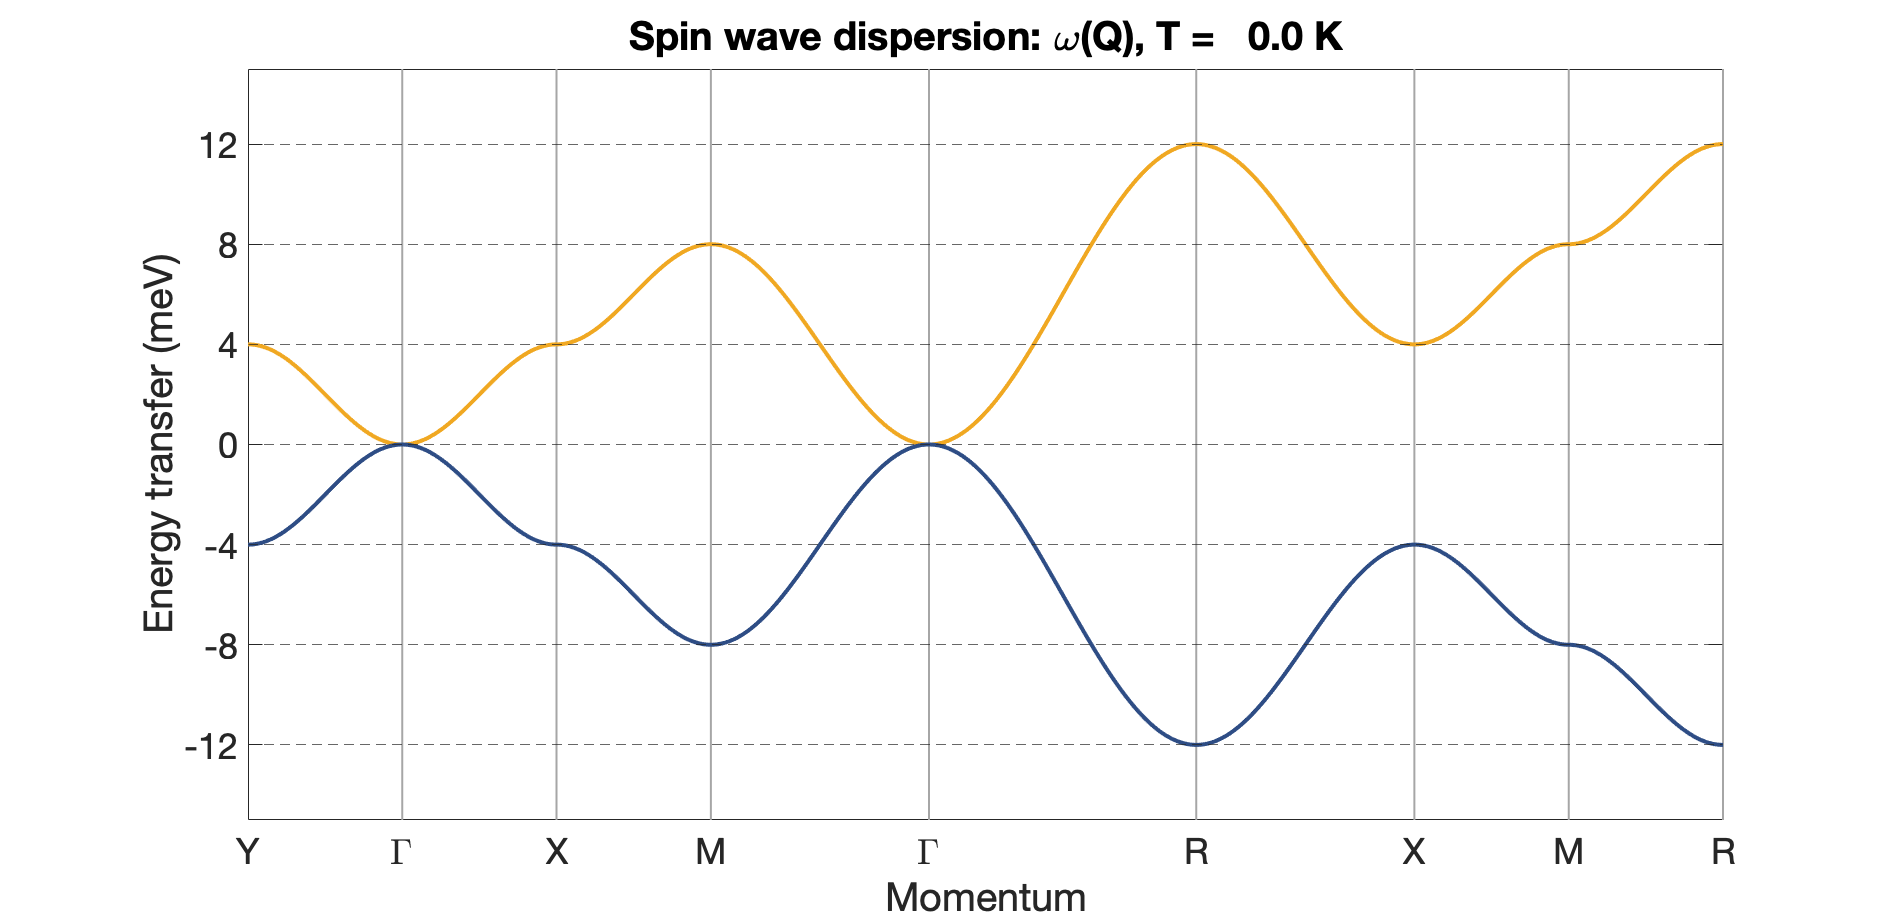
\includegraphics[height=7cm]{spinw-cub.png}
    %         \end{subfigure}
    %         \hfill
    %         \caption{Magnon dispersion plotted with SpinW.}
    %         \label{fig:spinw-cub}
    %     \end{figure}

    %     The sum over the Brillouin zone contains the $-\mathbf{k}$ vector for each $\mathbf{k}$ vector, 
    %     therefore the eq.\eqref{eq:spinw-cub} can be transformed to the desired form of the eq.~\eqref{eq:desired-form} (the constant energy shift is ignored here):
    %     \begin{equation}
    %         \begin{aligned}
    %             H = \sum_{\mathbf{k} \in B.Z.}\left(\hbar\omega_1(\mathbf{k})\hat{b}^{\dag}(\mathbf{k})\hat{b}(\mathbf{k}) 
    %             + \hbar\omega_1(-\mathbf{k})\hat{b}^{\dag}(\mathbf{-k})\hat{b}(\mathbf{-k})\right)\\ 
    %             = \sum_{\mathbf{k} \in B.Z.}\left(\hbar(\omega_1(\mathbf{k}) + \omega_1(\mathbf{k}))\hat{b}^{\dag}(\mathbf{k})\hat{b}(\mathbf{k})\right)
    %         \end{aligned}
    %     \end{equation}
    %     Which in the case of the cubic system leads to the same result as in eq.~\eqref{eq:main-dispersion} in the desired form of eq.~\eqref{eq:desired-form}:
    %     \begin{equation}
    %         \begin{aligned}
    %             H = \sum_{\mathbf{k} \in B.Z.}\left(\hbar\omega(\mathbf{k})\hat{b}^{\dag}(\mathbf{k})\hat{b}(\mathbf{k})\right)
    %         \end{aligned}
    %     \end{equation}
    %     where (in notation of SpinW)
    %     \begin{equation}
    %         \hbar\omega(\mathbf{k}) = 2\hbar \omega_1(\mathbf{k}) = 2SJn\left(\dfrac{1}{3}\left(\cos(k_xl) + \cos(k_yl) + \cos(k_zl)\right) - 1\right)
    %     \end{equation}

    %     However the SpinW code does plot the energies from eq.~\eqref{eq:spinw-cub}, but multiply the $\hbar\omega_1$ from the second term by $-1$. 
    %     In Fig.~\ref{fig:spinw-cub} the dispersion for the same path as in Fig.~\ref{fig:main-dispersion} is plotted. 
    %     The picture is produces with the script <<codes/spinw3D.m>>, which is based on the Tutorial 1 from the SpinW website (\url{https://www.spinw.org/tutorials/01tutorial})


    \begingroup
    \let\clearpage\relax
    \section{Appendix I}

In this section The magnon dispersion law is derived from the Hamiltonian in eq.~\eqref{eq:hh-main}.
First of all, the Hamiltonian is rewritten with the raising and lowering spin operators:

\begin{equation}
    \hat{S}_i^{\pm} = \hat{S}_i^x \pm \iu \hat{S}_i^y
\end{equation}

\begin{equation}
    \begin{matrix}
        \hat{\mathbf{S}}_i^T \hat{\mathbf{S}}_j = 
        \hat{S}_i^x \hat{S}_j^x + \hat{S}_i^y \hat{S}_j^y + \hat{S}_i^z \hat{S}_j^z; &
        \hat{S}_i^x \hat{S}_j^x + \hat{S}_i^y \hat{S}_j^y = 
        \dfrac{1}{2}\left(\hat{S}_i^+\hat{S}_j^- + \hat{S}_i^-\hat{S}_j^+\right)
    \end{matrix}
\end{equation}

\begin{equation}
    \hat{H} = -J \sum_{ij} \left(\dfrac{1}{2}\left(
        \hat{S}_i^+\hat{S}_j^- + \hat{S}_i^-\hat{S}_j^+\right) + \hat{S}_i^z \hat{S}_j^z\right)
\end{equation}

Since the commutator is 
\begin{equation}
    \left[\hat{S}_i^+\hat{S}_j^-\right] = 2\hat{S}_i^z\delta_{ij}
\end{equation}
and $i\ne j$ in the sum the Hamiltonian becomes:
\begin{equation}
    \hat{H} =-J \sum_{ij} \left(\dfrac{1}{2}\left(
            \hat{S}_j^-\hat{S}_i^+ + \hat{S}_i^-\hat{S}_j^+\right) + \hat{S}_i^z \hat{S}_j^z\right)
\end{equation}

The spin-wave Hamiltonian is obtained with the linearised Holstein–Primakoff formalism.

\begin{equation}
    \begin{matrix}
        \hat{S}_i^+ = \sqrt{2S}\hat{a}_i \\
        \hat{S}_i^- = \sqrt{2S}\hat{a}_i^{\dag} \\
        \hat{S}_i^z = S - \hat{a}_i^{\dag}\hat{a}_i
    \end{matrix}
\end{equation}

\begin{equation}
    \hat{H} = -J \sum_{ij} \left(\dfrac{1}{2}\left(
        2S\hat{a}_j^{\dag}\hat{a}_i + 2S\hat{a}_i^{\dag}\hat{a}_j\right) + 
        \left(S - \hat{a}_i^{\dag}\hat{a}_i\right)\left(S - \hat{a}_j^{\dag}\hat{a}_j\right)\right)
\end{equation}

\begin{equation}
    \hat{H} = E_0 + \hat{H}^{(2)} + \dots 
\end{equation}
\begin{equation}
    E_0 = -JS^2Nn \label{eq:zero-energy}
\end{equation}
\begin{equation}
    \hat{H}^{(2)} = -JS \sum_{ij} \left(\hat{a}_j^{\dag}\hat{a}_i + \hat{a}_i^{\dag}\hat{a}_j - 
    \hat{a}_i^{\dag}\hat{a}_i - \hat{a}_j^{\dag}\hat{a}_j\right)
    \label{eq:quadratic-ham}
\end{equation}
where $N$ is the number of spins in the system, $n$ - number of neighbors for each spin ($6$ in the case of cubic system).
From this point the quadratic part of the Hamiltonian $\hat{H}^{(2)}$ is considered.

The Fourier transform is introduced to move from the local operators $\hat{a}_i^{\dag}$ and $\hat{a}_i$
to the collective creation and annihilation operators $\hat{a}_k^{\dag}$ and $\hat{a}_k$:
\begin{equation}
    \hat{a}_i = \dfrac{1}{\sqrt{N}}\sum_k e^{\iu\mathbf{k}\mathbf{r}_i} \hat{a}_k 
\end{equation}
\begin{equation}
    \hat{a}_i^{\dag} = \dfrac{1}{\sqrt{N}}\sum_k e^{-\iu\mathbf{k}\mathbf{r}_i} \hat{a}_k^{\dag} 
\end{equation}
\begin{equation}
    \dfrac{1}{N}\sum_i e^{\iu(\mathbf{k} - \mathbf{k}^{\prime})\mathbf{r}_i} = \delta_{kk^{\prime}} 
\end{equation}

\begin{equation}
\begin{aligned}
    \hat{H}^{(2)}  = -JS \sum_i\sum_j \dfrac{1}{N}\left[
        \left(\sum_k e^{-\iu\mathbf{k}\mathbf{r}_j} \hat{a}_k^{\dag}\right)
        \left(\sum_{k^{\prime}} e^{\iu\mathbf{k^{\prime}}\mathbf{r}_i} \hat{a}_{k^{\prime}}\right)\right. \\
        +
        \left(\sum_k e^{-\iu\mathbf{k}\mathbf{r}_i} \hat{a}_k^{\dag}\right)
        \left(\sum_{k^{\prime}} e^{\iu\mathbf{k^{\prime}}\mathbf{r}_j} \hat{a}_{k^{\prime}}\right)  \\
        -
        \left(\sum_k e^{-\iu\mathbf{k}\mathbf{r}_i} \hat{a}_k^{\dag}\right)
        \left(\sum_{k^{\prime}} e^{\iu\mathbf{k^{\prime}}\mathbf{r}_i} \hat{a}_{k^{\prime}}\right)  \\
        -
        \left.\left(\sum_k e^{-\iu\mathbf{k}\mathbf{r}_j} \hat{a}_k^{\dag}\right)
        \left(\sum_{k^{\prime}} e^{\iu\mathbf{k^{\prime}}\mathbf{r}_j} \hat{a}_{k^{\prime}}\right) \right]
\end{aligned}
\end{equation}

Since for each $i$ there is the same pattern of neighbors sum over $j$ does not depend on $i$ and it can be moved freely.
Lets define $\boldsymbol{\delta}_j = \mathbf{r}_j - \mathbf{r}_i$ and rewrite the equation:

\begin{equation}
\begin{aligned}
    \hat{H}^{(2)}  = -JS \sum_k\sum_{k^{\prime}}\sum_j \left[
        e^{-\iu\boldsymbol{\delta}_j\mathbf{k}}
        \left(\dfrac{1}{N}\sum_ie^{\iu(\mathbf{k^{\prime}}-\mathbf{k})\mathbf{r}_i}\right) 
        \hat{a}_k^{\dag}\hat{a}_{k^{\prime}}\right. \\
        +
        e^{\iu\boldsymbol{\delta}_j\mathbf{k}}
        \left(\dfrac{1}{N}\sum_ie^{\iu(\mathbf{k^{\prime}}-\mathbf{k})\mathbf{r}_i}\right)
         \hat{a}_k^{\dag}\hat{a}_{k^{\prime}}  \\
        -
        \left(\dfrac{1}{N}\sum_ie^{\iu(\mathbf{k^{\prime}}-\mathbf{k})\mathbf{r}_i}\right)
        \hat{a}_k^{\dag}\hat{a}_{k^{\prime}}  \\
        -
        \left.e^{\iu(\mathbf{k^{\prime}}-\mathbf{k})\boldsymbol{\delta}_j}
        \left(\dfrac{1}{N}\sum_ie^{\iu(\mathbf{k^{\prime}}-\mathbf{k})\mathbf{r}_i}\right)
        \hat{a}_k^{\dag}\hat{a}_{k^{\prime}} \right]
\end{aligned}
\end{equation}
every equation in round parenthesis is equal to $\delta_{kk^{\prime}}$ and the Hamiltonian becomes

\begin{multline}
    \hat{H}^{(2)} = -JS\sum_k\sum_j\left[e^{-\iu\boldsymbol{\delta}_j\mathbf{k}}
    \hat{a}_k^{\dag}\hat{a}_k
    +
    e^{\iu\boldsymbol{\delta}_j\mathbf{k}}
     \hat{a}_k^{\dag}\hat{a}_k 
    -
    \hat{a}_k^{\dag}\hat{a}_k 
    -
    e^{\iu(\mathbf{k}-\mathbf{k})\boldsymbol{\delta}_j}
    \hat{a}_k^{\dag}\hat{a}_k\right] \\
     = 2JS\sum_k\sum_j(1 - \cos(\boldsymbol{\delta}_j\mathbf{k}))\hat{a}_k^{\dag}\hat{a}_k
\end{multline}
$j$ runs from $1$ to $n$, therefore:
\begin{equation}
    \hat{H}^{(2)} = 2JSn\sum_k\left(1 - \dfrac{1}{n}\sum_j
    \cos(\boldsymbol{\delta}_j\mathbf{k})\right)\hat{a}_k^{\dag}\hat{a}_k = 
    \sum_k \hbar\omega(\mathbf{k})\hat{a}_k^{\dag}\hat{a}_k
\end{equation}

For the cubic system ($l$ - length of the lattice vector):
\begin{align}
    \dfrac{1}{n}\sum_j
    e^{\iu\boldsymbol{\delta}_j\mathbf{k}}  = \dfrac{1}{6}\left(\cos(k_xl) + \cos(-k_xl) + \cos(k_yl) + \cos(-k_yl) + \cos(k_zl) + \cos(-k_zl)\right) \\
    = \dfrac{1}{3}\left(\cos(k_x l) + \cos(k_y l) + \cos(k_z l)\right)
\end{align}
and the final formula for the magnon dispersion is
\begin{equation}
    \hbar\omega(\mathbf{k}) = 2JSn\left(1 - 
    \dfrac{1}{3}\left(\cos(k_x l) + \cos(k_y l) + \cos(k_z l)\right)\right)
\end{equation}
    \endgroup

    \bibliographystyle{plain} 
    \bibliography{refs.bib} 


    % \section*{References}
    % \printbibliography[title = {\vspace{-2em}}]



\end{document}
